\chapter{Virtual-Vertigo} \label{vertigo}
Ce chapitre décrit de manière plus détaillée le projet \textit{Virtual-Vertigo}. Il est séparé en deux parties distinctes, un descriptif du dispositif et la présentation de  l'architecture de l'application. Ces parties sont illustrées afin d'en faciliter la compréhension.

%%%%%%%%%%%%%%%%%%%%%%%%%%%%%%%%%%%%%%%%%%%%%%%%%%%%%%%%%%%%%%%%%%%%%%%%%%%%%%%%%%%%%%%%%%%%%%%%%%%%%%%%%%%%%%%%%%%%%%%%%%%

\section{Dispositif} \label{dispositif}

Le projet \textit{Virtual-Vertigo} aide une personne à combattre sa peur du vide en utilisant la réalité virtuelle. Pour cela, cette personne portera un casque de réalité virtuelle constitué d'un téléphone et d'un support en carton comprenant des lentilles. Ce dispositif permet l'affichage d'une scène virtuelle 3D via des images stéréoscopiques. \\
Lors de la simulation, l'utilisateur devra avancer sur une planche placée au sol. Un appareil posé sur une table face à la planche permettra de capturer ses mouvements. L'appareil connecté à un serveur devra transmettre les informations de positions au téléphone. Un affichage sur un écran standard donnera aussi une autre vue de la scène.\\

Voici quelques images illustrant la vue de la scène :
\begin{figure}[H]
   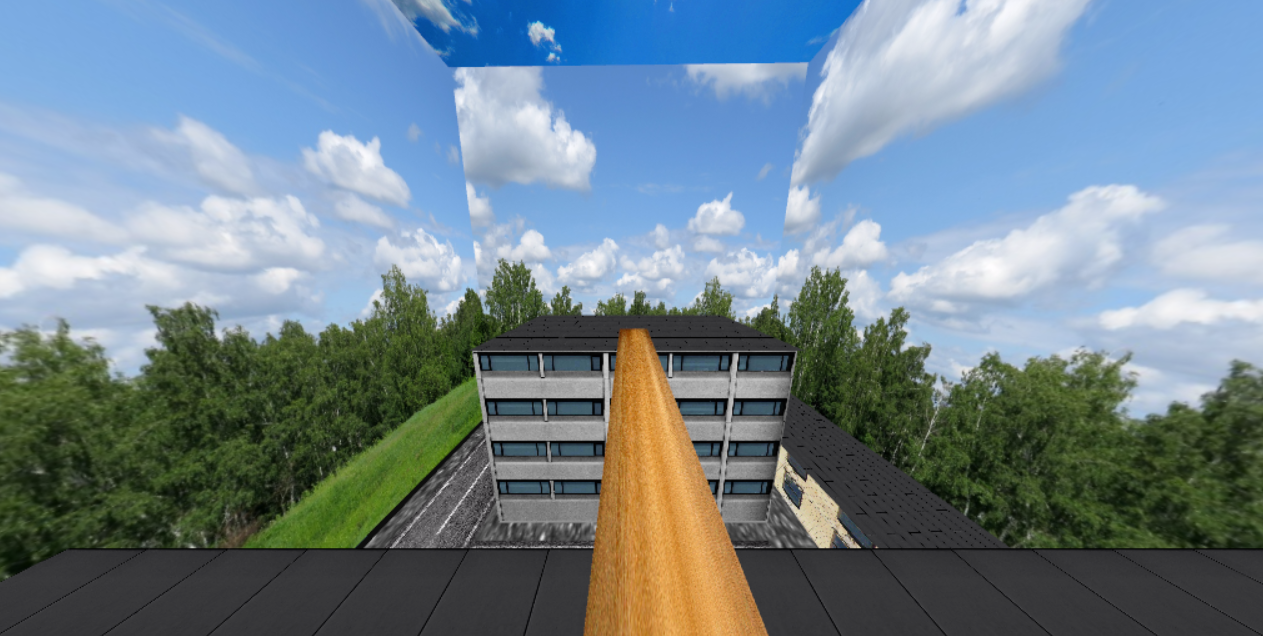
\includegraphics[scale=0.202]{vueBasiqueTextures.png}
   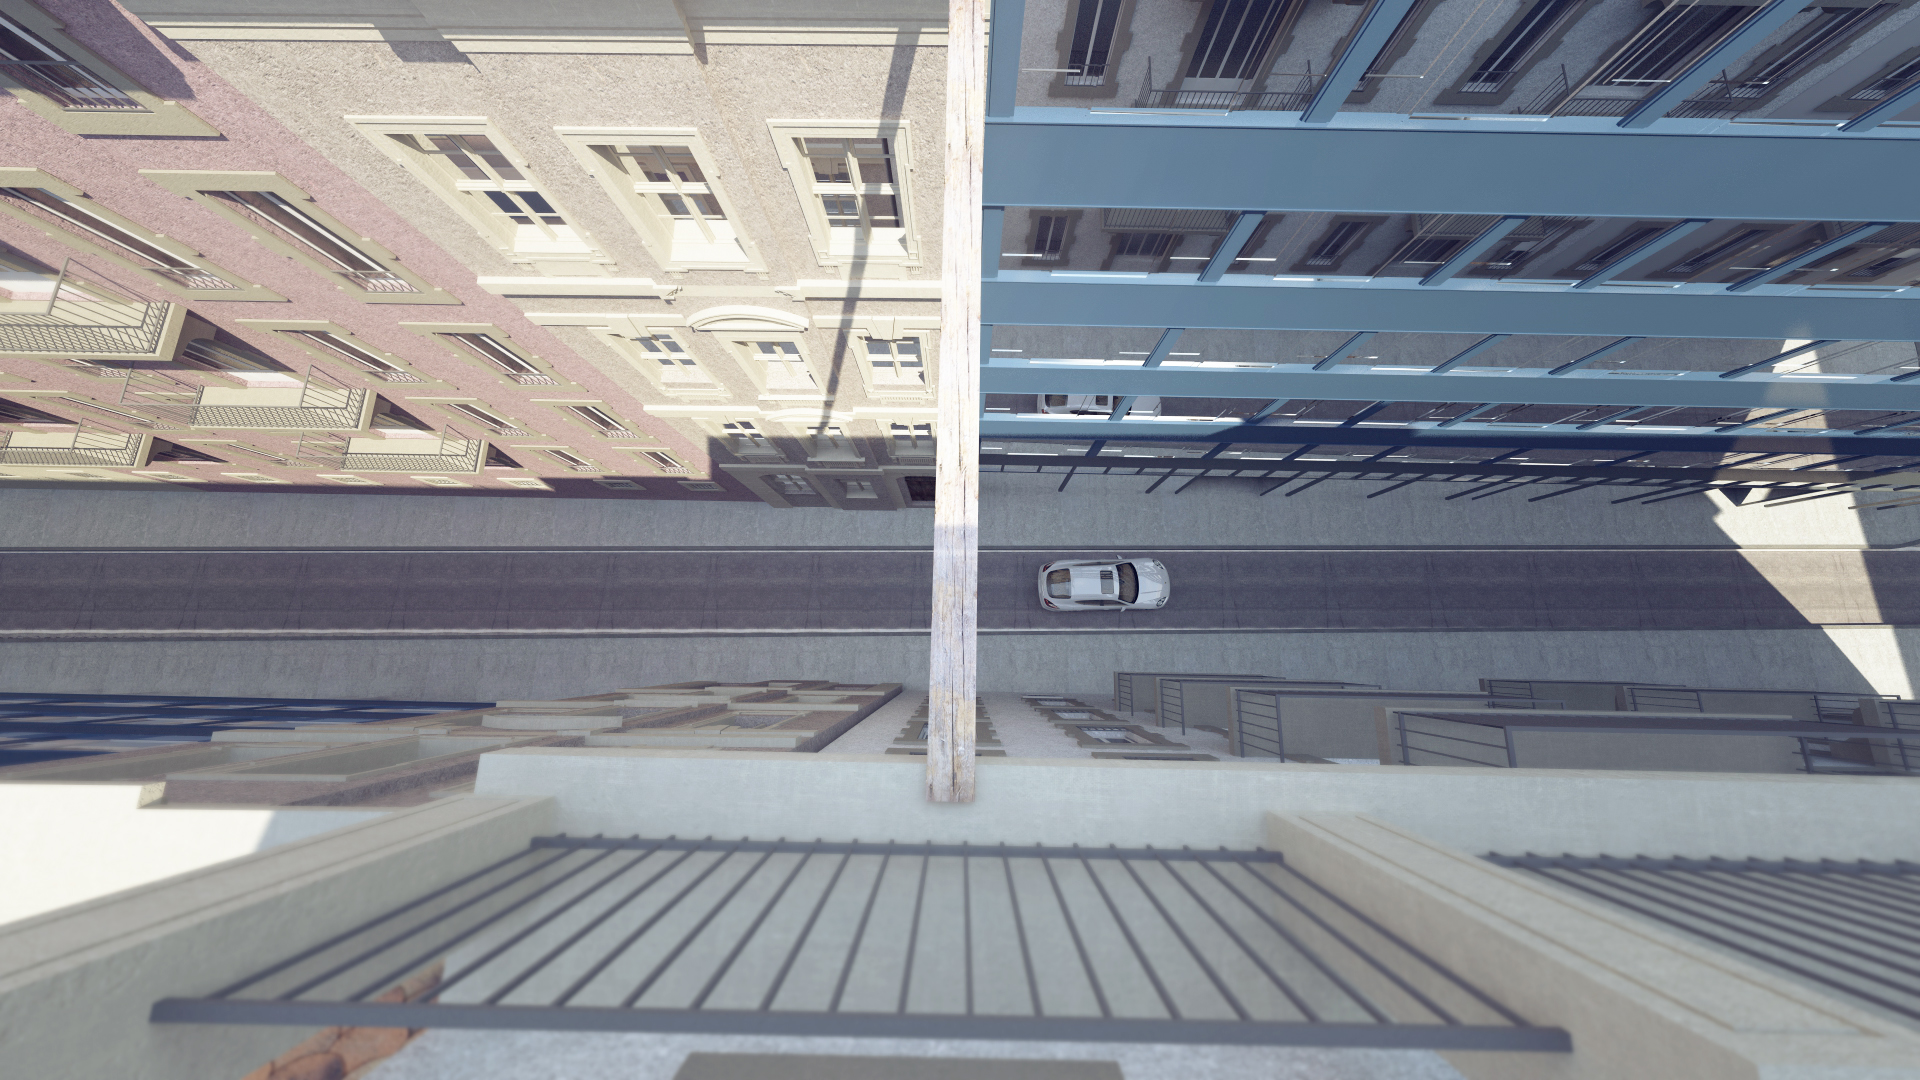
\includegraphics[scale=0.09]{Vue_planche2_ok.jpg}
   \caption{\label{vue} Vue 3D vue par la personne portant les lunettes}
\end{figure}

La deuxième image a été produite par \textsc{M. Benjamin Dupond-Roy}, assistant à hepia en filière architecture du paysage. Plus d'informations sont disponibles quant à la construction de ces images à la section~\ref{realiteVirtuelle}.

A noter qu'un tutoriel contenant les instructions pour l'installation et l'utilisation du projet \textit{Virtual-Vertigo} est disponible en annexe.

%%%%%%%%%%%%%%%%%%%%%%%%%%%%%%%%%%%%%%%%%%%%%%%%%%%%%%%%%%%%%%%%%%%%%%%%%%%%%%%%%%%%%%%%%%%%%%%%%%%%%%%%%%%%%%%%%%%%%%%%%%%

\subsection*{Composants} \label{composants}
Ci-dessous se trouve la liste des appareils et logiciels utilisés dans le projet : 

\begin{itemize}
\item \textbf{une Google CardBoard} : il s'agit du casque de réalité virtuelle en carton et équipé de lentilles;
\item \textbf{un smartphone} : il s'agit de l'appareil qui permet la visualisation en 3D stéréoscopique;
\item \textbf{un Kinect version 1} : c'est l'appareil qui détecte les mouvements de la personne sur la planche; 
\item \textbf{Kinect SDK 1.8} : c'est le logiciel permettant d'utiliser le \textit{Kinect} à partir d'un ordinateur;
\item \textbf{NodeJS} : c'est le \textit{Framework JavaScript} permettant de créer et lancer le serveur qui gère les transmissions entre le \textit{Kinect} et les clients HTML (\textsf{smartphone}, PC, etc.);
\item \textbf{un ordinateur sur Windows 7 ou plus} : il s'agit du serveur sur lequel est connecté le \textit{Kinect}. \\

\end{itemize}

Le schéma suivant illustre l'interaction entre les composants mentionnés ci-dessus. Sous chaque composant se trouvent les technologies qu'il utilise.\\

\begin{figure}[H]
	\centering
   		\includegraphics[scale=0.3]{description.png}
   \caption{\label{Schéma} Schéma du projet et de ses composants}
\end{figure}

La description de chaque composant est donnée au chapitre~\ref{implementation}. \\
A noter également qu'un glossaire décrivant toutes les technologies et les outils utilisés dans le projet \textit{Virtual-Vertigo} est disponible en annexe.

\subsubsection{Prix des composants}
Les seuls composants devant être achetés sont le \textit{Kinect} et les \textit{Google CardBoard}, le \textsf{smartphone} n'est pas pris en compte dans la liste des achats car tout le monde en possède un. Voici un tableau des prix :

\begin{center}
	\begin{tabular}{| c | c |}
	\hline
		\textbf{Composant} & \textbf{Prix} \\ \hline
		Kinect v1 pour Windows & 150 CHF \\ \hline
		Google CardBoard à assembler & 11 CHF \\ \hline
		Matériel pour les Google CardBoard & 11 CHF \\ \hline
		Kinect v2 + adaptateur pour Windows & 180 CHF \\ \hline
		Occulus Rift & entre 300 et 400 CHF\\ \hline
	\end{tabular} 
	\captionof{table}{\label{prix}Tableau prix des composants}
\end{center}

Le tableau~\ref{prix} montre que le prix total des composants nécessaires au projet \textit{Virtual-Vertigo} est de moins de 200 CHF. Si l'\textit{Occulus Rift} avait été utilisé au lieu des \textit{Google CardBoard} le prix du projet aurait triplé. Le prix des \textit{Occulus Rift} est économisé. 

%%%%%%%%%%%%%%%%%%%%%%%%%%%%%%%%%%%%%%%%%%%%%%%%%%%%%%%%%%%%%%%%%%%%%%%%%%%%%%%%%%%%%%%%%%%%%%%%%%%%%%%%%%%%%%%%%%%%%%%%%%%
\subsection*{Disposition générale des composants} \label{disposition}
Le projet utilise beaucoup de composants qui doivent être positionnés de manière précise. Le schéma suivant montre l'emplacement de chaque composant.

\begin{figure}[H]
	\centering
   		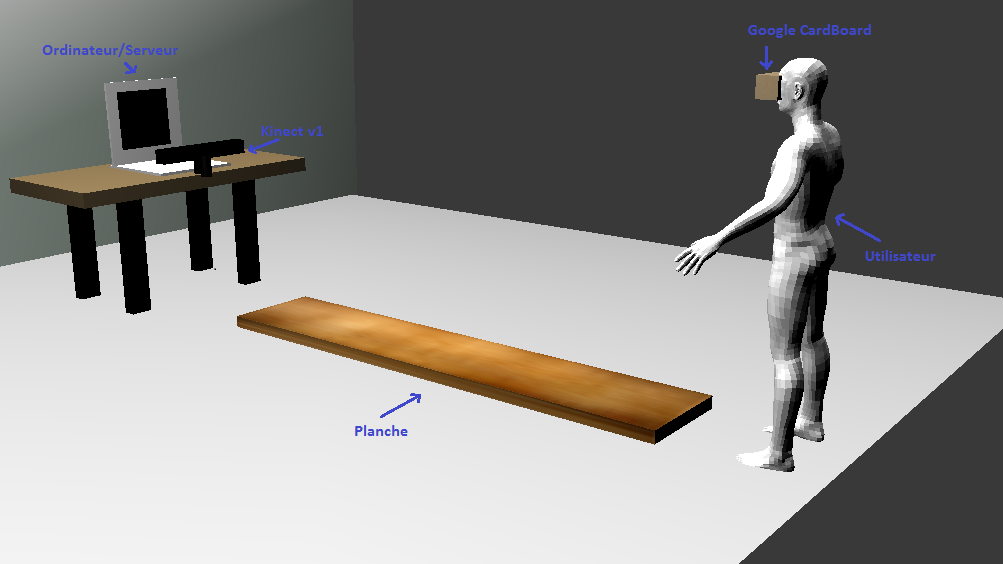
\includegraphics[scale=0.5]{vertigo.png}
   	\caption{\label{vertigo} Modèle 3D de l'installation de \textit{Virtual-Vertigo}}
\end{figure}

Ce schéma ne montre cependant pas les restrictions imposées par le \textit{Kinect}: 
\begin{itemize}
\item la planche placée sur le sol ne peut pas faire plus de 3 mètres;
\item la planche doit être placée à une distance d'au moins 80 centimètres du \textit{Kinect};
\item l'utilisateur doit se trouver à une distance de moins de 4 mètres du \textit{Kinect};
\item le \textit{Kinect} doit être placé au bord de la table afin d'éviter qu'il ne capte pas les membres inférieurs de l'utilisateur ;
\item le \textit{Kinect} doit être connecté en USB à l'ordinateur. \\

\end{itemize}

A noter que le \textsf{smartphone} est connecté en wifi ou 3G au serveur. Il est intégré aux \textit{Google CardBoard} et affiche chacune des deux images stéréoscopiques que l'utilisateur visualise à travers les lentilles.\\

Les photos~\ref{reelle} sont l'installation réelle mise en place durant le développement du projet \textit{Virtual-Vertigo}.
\begin{figure}[H]
\centering
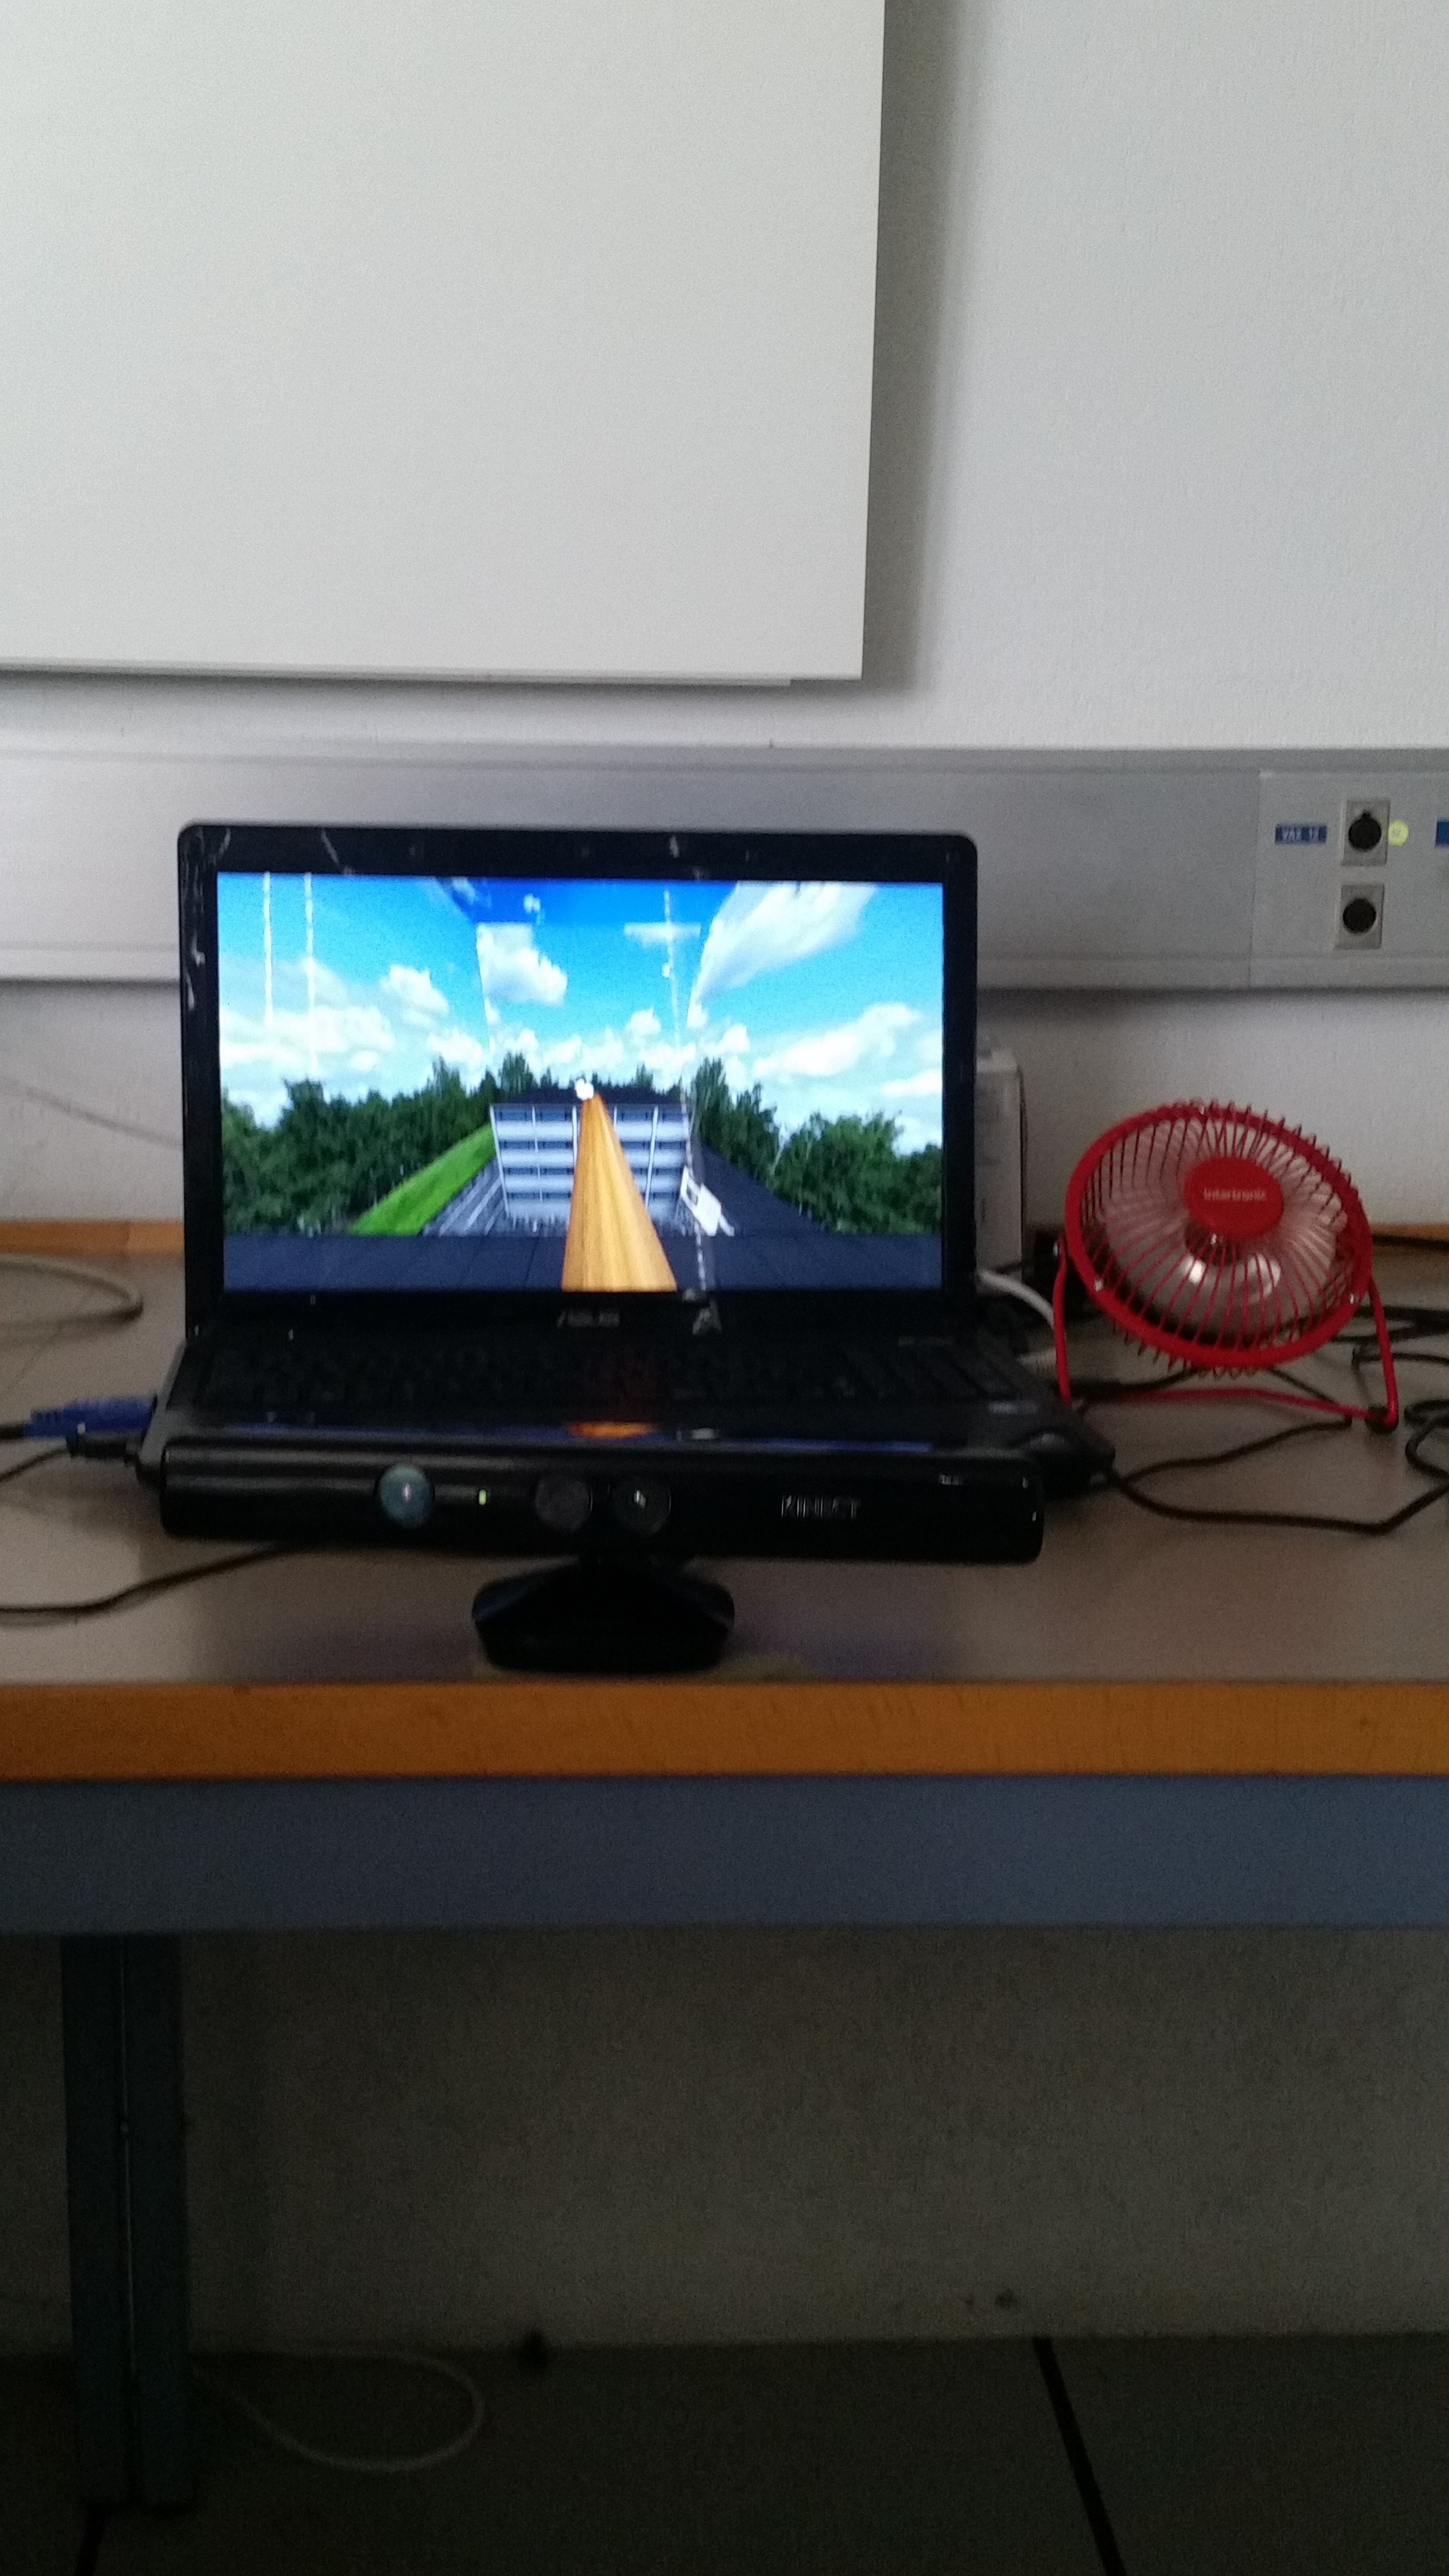
\includegraphics[scale=0.04]{vueReelle2.jpg}
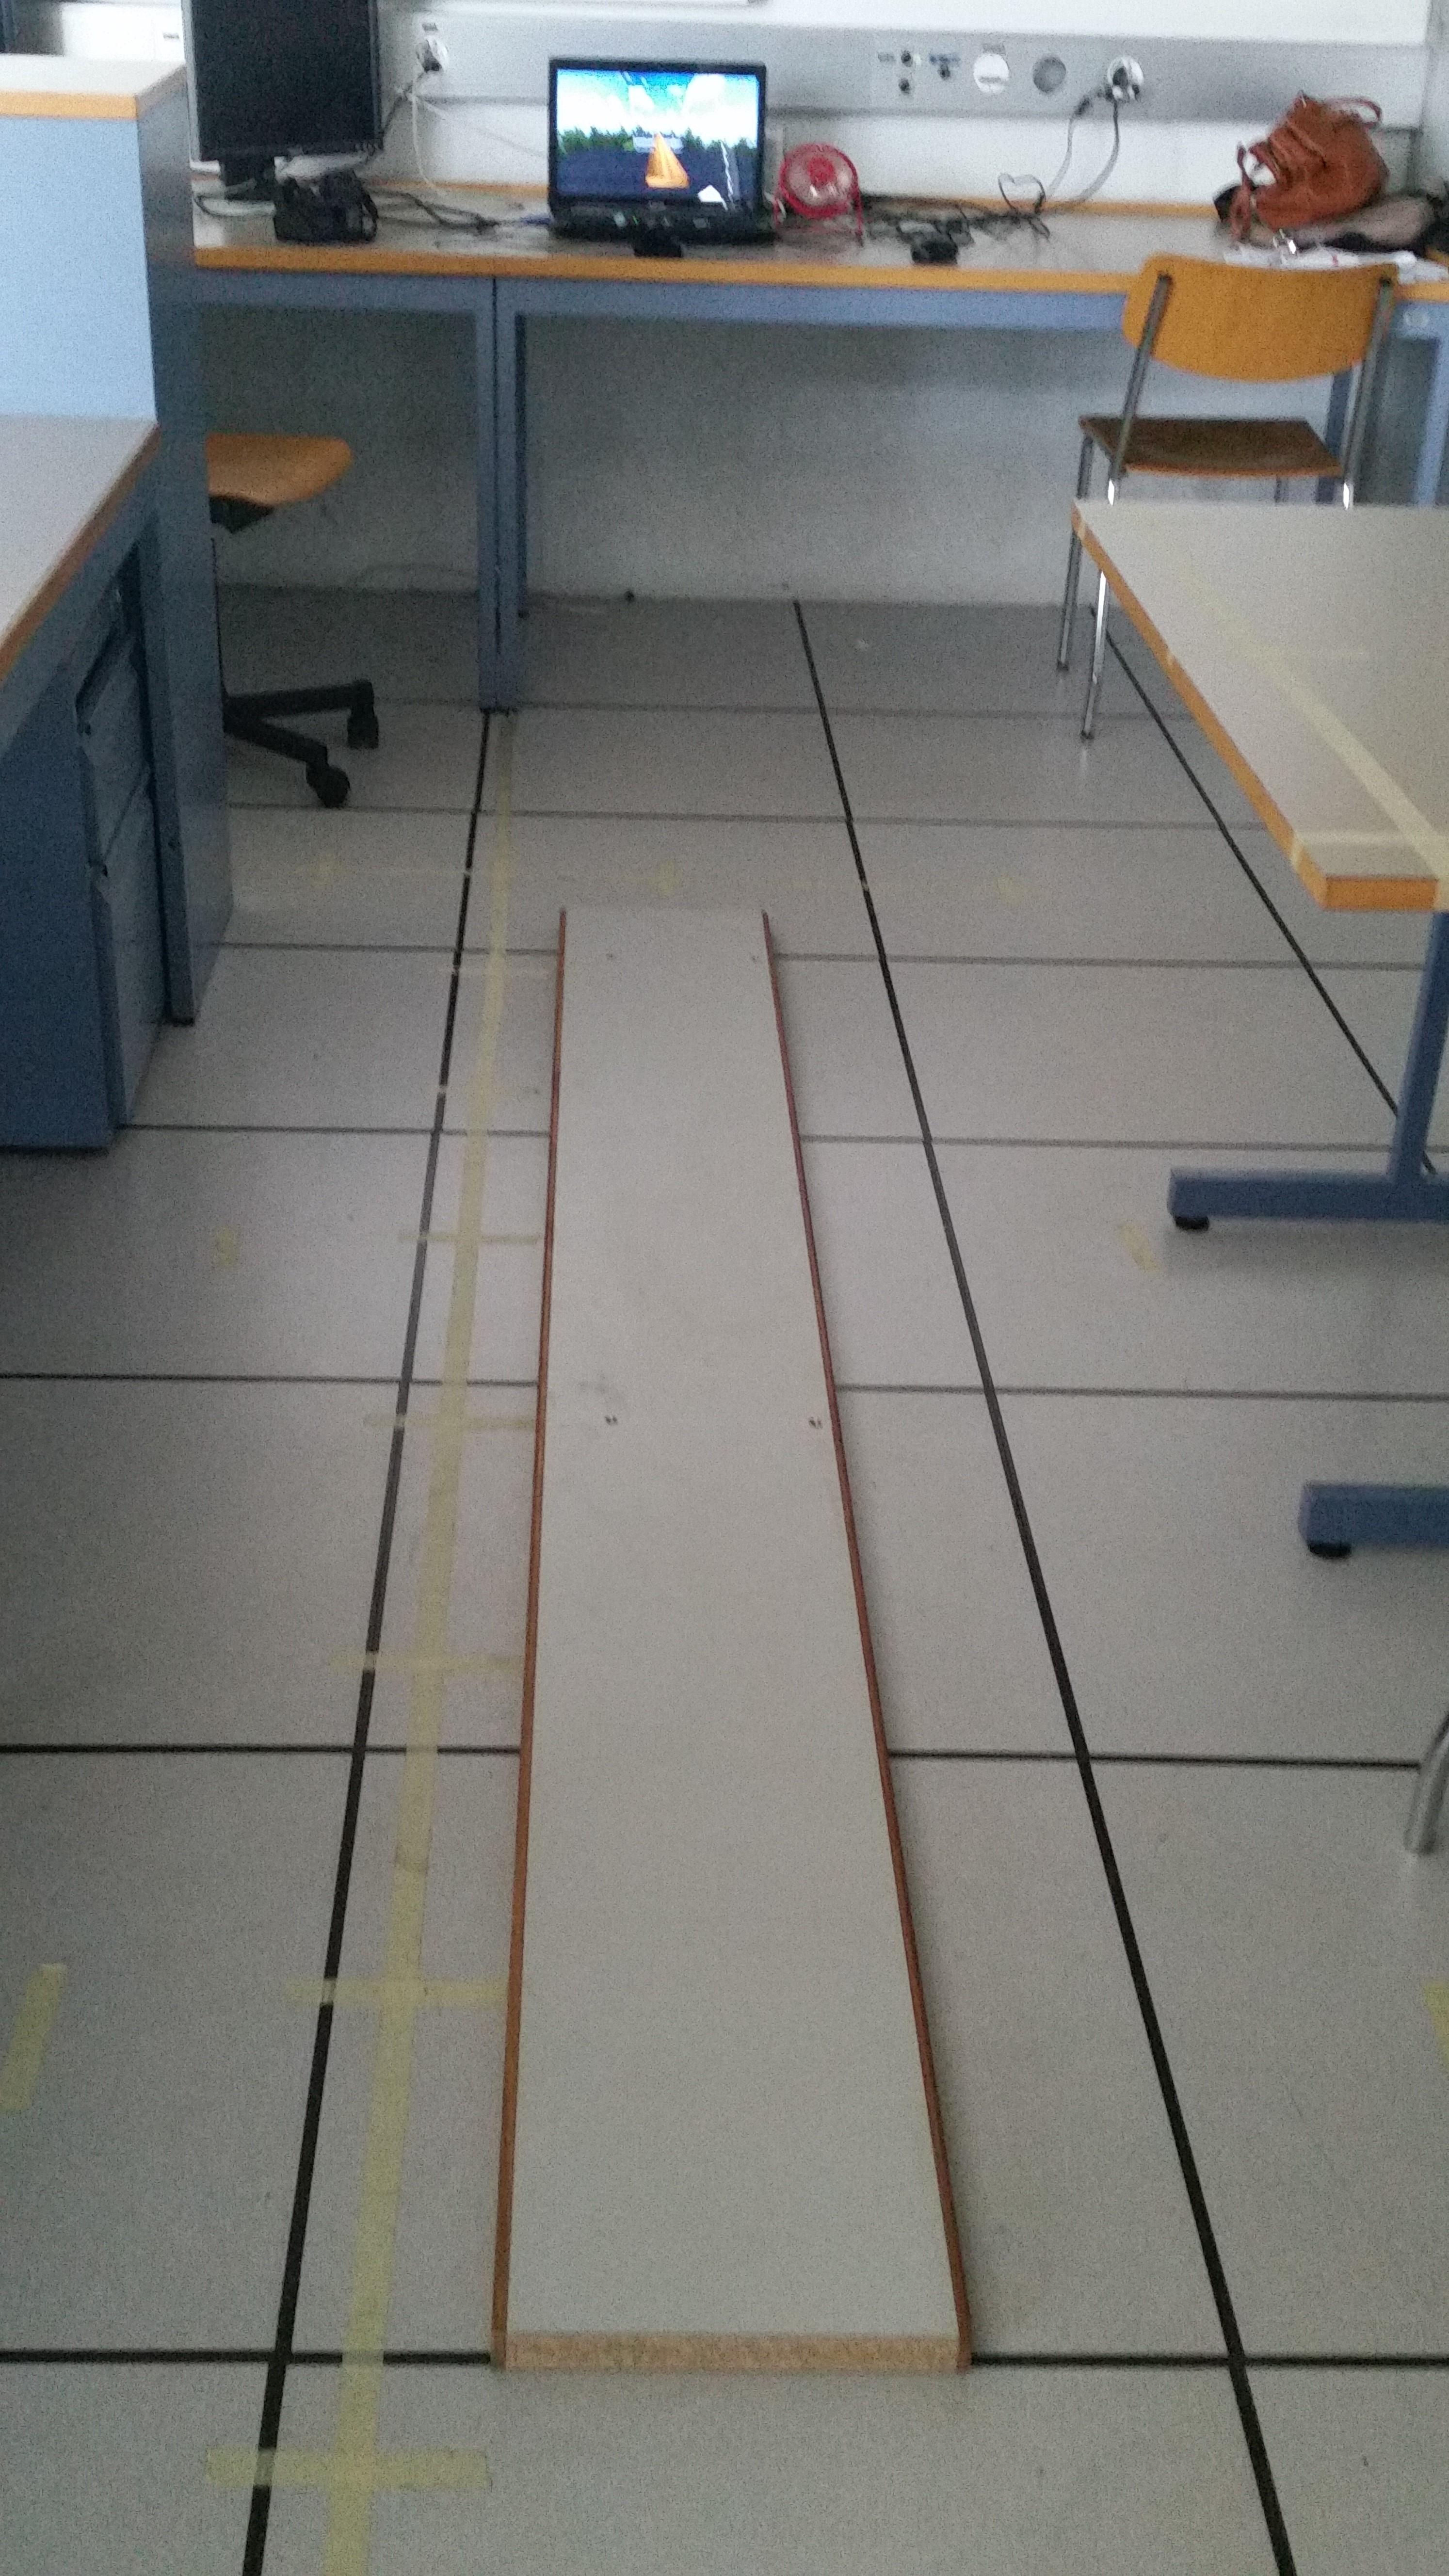
\includegraphics[scale=0.04]{vueReelle3.jpg}
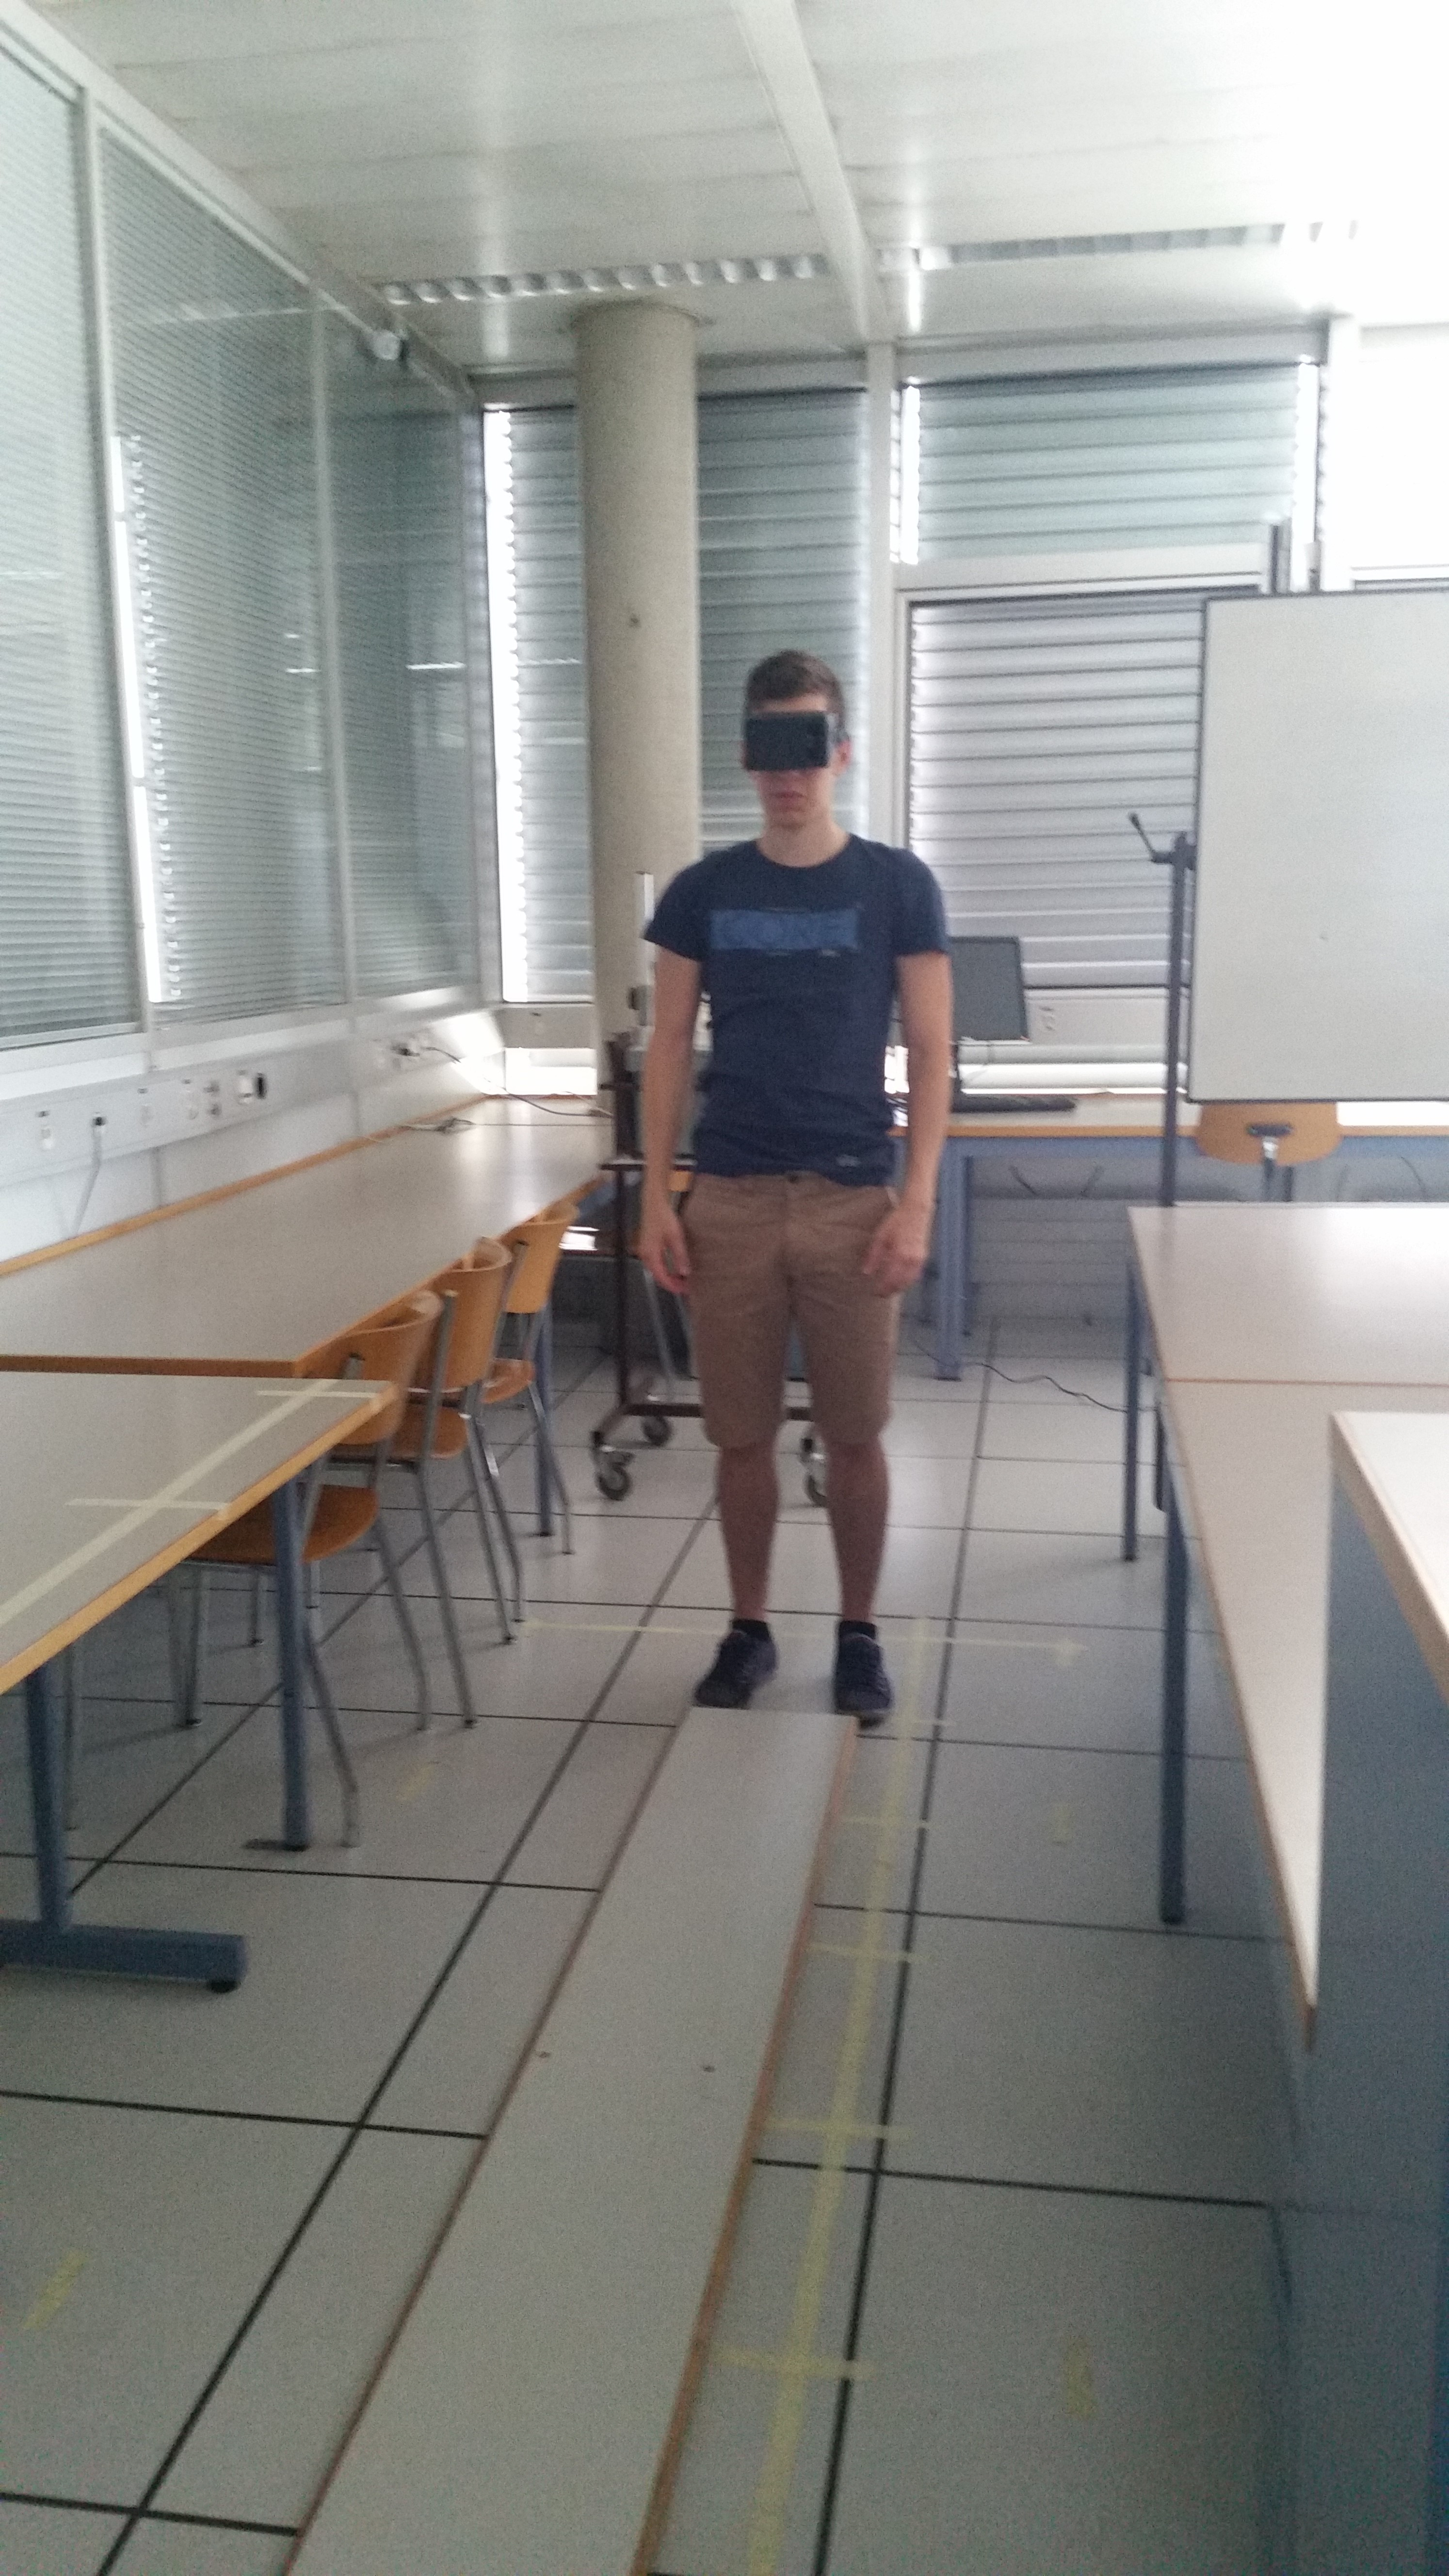
\includegraphics[scale=0.04]{vueReelle1.jpg}
\caption{\label{reelle} Illustrations de l'installation réelle mise en place}
\end{figure}

%%%%%%%%%%%%%%%%%%%%%%%%%%%%%%%%%%%%%%%%%%%%%%%%%%%%%%%%%%%%%%%%%%%%%%%%%%%%%%%%%%%%%%%%%%%%%%%%%%%%%%%%%%%%%%%%%%%%%%%%%%%

\subsection*{Effets de réalisme}  \label{realisme}
Le réalisme est très important dans ce projet. C'est pour cela que l'utilisation de quelques objets est mis en place afin de plonger la personne dans la situation la plus réaliste possible. Une planche et un effet sonore ont été ainsi ajoutés au projet.\\

\subsubsection{Planche}
Pour le ressenti de la planche sous les pieds, une planche de 2,50 mètres de distance ayant environ 5 centimètres d'épaisseur a été mise en place. Cette planche va permettre à la personne de sentir les bords de la planche quand elle s'en approche et donc d'avoir la sensation de déséquilibre et de "chute" possible. 

\subsubsection{Effet sonore environnant}
Lorsque l'utilisateur se trouve sur le toit d'un immeuble, il y a également tous les bruits environnants quotidiens, comme par exemple, les klaxons, les voitures qui passent, les gens qui parlent ou même les oiseaux. Un enregistrement des bruits sonores ambiant peut être effectué, lequel se déclencherait lorsque la personne atteint le bout de la planche. Pour cela, on envisage deux solutions possibles : \\

\begin{itemize}
\item un casque \textsf{bluetooth} qui sera connecté à l'ordinateur;
\item le \textsf{smartphone} lui-même.\\

\end{itemize}

Cette amélioration a été mise en place en utilisant le casque \textsf{bluetooth} car sur le \textsf{smartphone} il est impossible de déclencher la bande sonore sans avoir un \textsf{touch event}. \\
Ce dernier cas  sur \textsf{smartphone} n'a pas été envisagé pour une question de temps. Sinon, la bande peut être lancée lorsque la vue est mise en \textsf{fullscreen} manuellement. Le volume serait désactivé tant que  la personne n'atteint pas le bout de la planche.

\subsubsection{Sensation de vent}
Sur le toit d'un immeuble, il y a souvent du vent. C'est pour cette raison qu'un ventilateur peut être ajouté afin que l'utilisateur ressente le vent lors de l'exercice.

\subsubsection{Pulsations cardiaques}
Afin de pouvoir comparer les résultats des différentes tentatives et donc savoir si le système permet bien de vaincre la peur du vide, une montre connectée peut être utilisée. L'utilisateur devrait alors la porter lors de l'exercice. Cette montre communiquerait au serveur via le \textsf{smartphone} les informations cardiaques. Ces informations seraient stockées dans une base de données ou dans un fichier pour le suivi de l'évolution.\\
Elle permettrait également de contrôler en temps réel la personne en cas de crise ou tout autre problème physique. \\

%%%%%%%%%%%%%%%%%%%%%%%%%%%%%%%%%%%%%%%%%%%%%%%%%%%%%%%%%%%%%%%%%%%%%%%%%%%%%%%%%%%%%%%%%%%%%%%%%%%%%%%%%%%%%%%%%%%%%%%%%%%

\pagebreak
\section{Architecture}  \label{architecture}
L'architecture du projet est importante car elle permet d'avoir une application structurée et complète. L'architecture d'un projet consiste à décrire utilisant des schémas, des graphiques et des diagrammes le projet. Ici, elle contient l'organisation, la description du déroulement du projet et la description de la communication entre chaque composant présent. \\
 
Ici, l'organisation consiste à structurer en plusieurs classes ou fichiers. La séparation permet d'avoir une application mieux organisée et modulaire. Cette organisation est décrite dans la figure suivante :
\begin{figure}[H]
	\centering
   		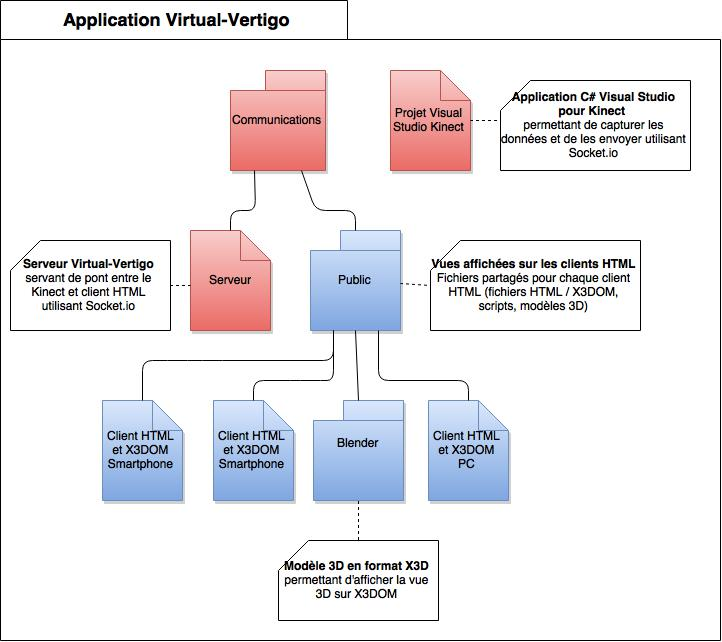
\includegraphics[scale=0.67]{Architecture.jpg}
   	\caption{\label{architecture} Architecture du projet \textit{Virtual-Vertigo}}
\end{figure}

\begin{itemize}
\item \textbf{Projet Visual Studio Kinect} : il s'agit de l'application C\# Visual Studio du \textit{Kinect}. Cette application capte les mouvements de l'utilisateur et envoie les positions aux clients via le module de communication \textit{Socket.io};
\item \textbf{Communications} : il s'agit d'un dossier contenant les fichiers privés de l'application qui gèrent la communication. Ce dossier contient aussi les fichiers nécessaires au fonctionnement du serveur;
\item \textbf{Serveur} : il s'agit du \textit{serveur Web Virtual-Vertigo}. Ce serveur correspond au pont entre le \textit{Kinect} et les clients HTML;
\item \textbf{Public} : c'est le dossier contenant les fichiers publics de l'application. Ce dossier contient les pages HTML, les scripts et les modèles 3D; 
\item \textbf{Script} : il s'agit du script modifiant la scène 3D. Ce script réceptionne les positions, crée le personnage virtuel, anime les membres de ce personnage et déplace ce personnage sur la planche;
\item \textbf{Client HTML et X3DOM Smartphone} : c'est le fichier HTML contenant la scène stéréoscopique 3D;
\item \textbf{Blender} : c'est le dossier contenant les modèles 3D ainsi que leurs textures;
\item \textbf{Client HTML et X3DOM PC} : c'est le fichier HTML contenant la scène non stéréoscopique 3D affichée sur un écran standard.\\ \linebreak
 
\end{itemize} 

A noter que les éléments en rouge sont des éléments privés que seul la personne s'occupant du serveur peut avoir accès. Les éléments en bleu contiennent les éléments publiques. C'est-à-dire, les clients HTML (\textsf{smartphone} et PC), les scripts JavaScript interagissant avec la vue et les modèles 3D. Plus de détails sur ces composants logiciels sont donnés au chapitre~\ref{implementation}.\\

 
La description du déroulement du projet consiste, via un diagramme ou un schéma, à montrer la vie du projet. C'est à dire, décrire ce qu'il se passe entre chaque événement et comment le changement d'événement s'effectue. Le déroulement du projet est illustré par le diagramme de séquence~\ref{sequence} :
\begin{figure}[H]
	\centering
   		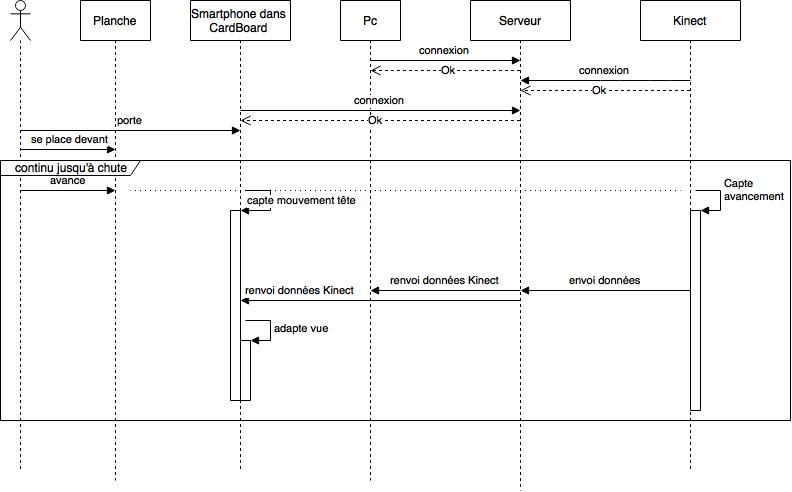
\includegraphics[scale=0.6]{VertigoSequence.jpg}
   	\caption{\label{sequence} Diagramme de séquence du projet \textit{Virtual-Vertigo}}
\end{figure}

Ce diagramme montre deux phases : l'une d'initialisation, et l'autre de simulation. L'initialisation correspond au lancement du serveur, puis la connexion du \textsf{smartphone} et du \textit{Kinect} à ce serveur. La phase de simulation commence quand l'utilisateur se place devant la planche. Une fois la simulation démarrée, les opérations suivantes sont effectuées en boucle : 

\begin{itemize}
\item le Kinect capte les mouvements de la personne;
\item le Kinect transmet les positions au serveur;
\item le serveur retransmet ces positions aux clients HTML connectés;
\item Les clients HTML adaptent leurs vues.\\

\end{itemize}
Cette boucle s'exécute toutes les secondes et s'arrête quand la personne "chute" ou quand elle arrive au bout de la planche.\\

Le déroulement du projet peut également être détaillé en se basant sur les différents états durant la simulation. Le diagramme~\ref{activiteDiag} montre les états des composants du projet et l'action qui les fait changer d'état.
\begin{figure}[H]
	\centering
   		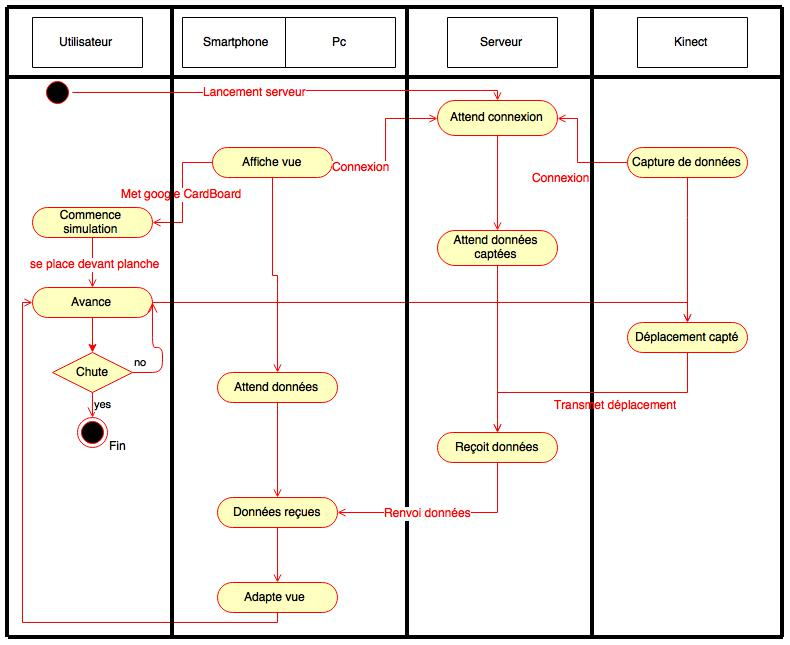
\includegraphics[scale=0.6]{VertigoActivite.jpg}
   	\caption{\label{activiteDiag} Diagramme d'activité du projet \textit{Virtual-Vertigo}}
\end{figure} 
L'application commence par le lancement du serveur qui se met en attente d'une connexion d'un client. Lorsque le \textit{Kinect} et les clients HTML se connectent, le serveur attend de recevoir les positions captées par le \textit{Kinect} pour ensuite les retransmettre aux clients HTML. Lors de la réception des positions, les clients adaptent la vue virtuelle. En parallèle, l'utilisateur effectue sa simulation de réalité virtuelle.




